%
% radonft.tex
%
% (c) 2023 Prof Dr Andreas Müller
%
\begin{figure}
\centering
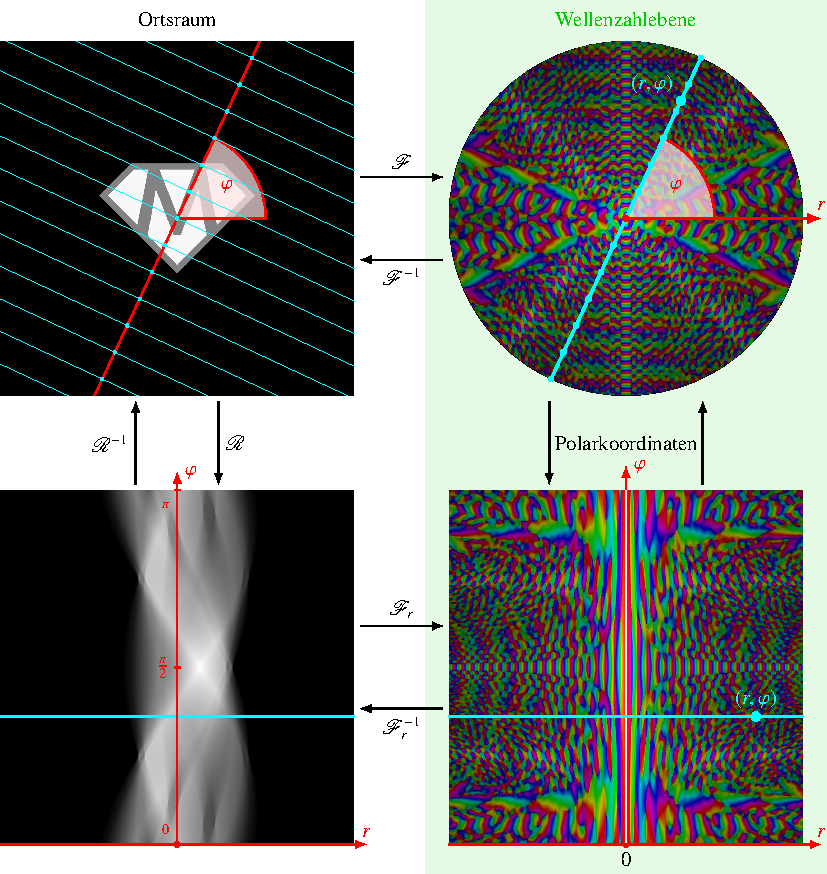
\includegraphics[width=\textwidth]{chapters/050-radon/images/radonft.pdf}
\caption{Zusammenspiel der Radon- und Fourier-Transformation.
Die Radontransformation $\mathscr{R}$ gefolgt von einer (radialen)
Fourier-Transformation $\mathscr{F}_r$, die nur die $r$-Koordinate
betrifft, wird zur einer Fourier-Transformation $\mathscr{F}$, wenn
man die $(r,\varphi)$ als Polarkoordinaten der Wellenzahl-Ebene
(rechte Hälfte der Abbildung) interpretiert.
\label{buch:radon:definition:fig:radonft}}
\end{figure}
